%% hack to load amsfonts instead of amssymb to properly make hbar bold
\RequirePackage{scrlfile}
\makeatletter
\AfterPackage{beamerbasemodes}{\beamer@amssymbfalse}
\makeatother
\documentclass[xcolor={svgnames,rgb}]{beamer}
\let\oldhbar\hbar
\usepackage{amssymb}
\def\hbar{\boldsymbol{\oldhbar}}

%%other packages
\usepackage{braket}

%% fonts

\usepackage[no-math]{fontspec}
\setmainfont[Mapping=tex-text,Numbers={Lining}]{Hoefler Text}
%\setmainfont[Mapping=tex-text]{Optima}
\usepackage[SlantFont]{xeCJK}
%\setCJKmainfont{Hiragino Maru Gothic Pro}
\setCJKmainfont{Hiragino Mincho Pro}
%\setCJKmainfont{Hiragino Sans W2}
\setCJKfamilyfont{tt}{Hiragino Maru Gothic Pro}




%% colors

\definecolor{myblue}{HTML}{100080}
\definecolor{math}{HTML}{100080}
\definecolor{blendedblue}{rgb}{0.2,0.2,0.7}

\def\bff{\ifmmode\else\bfseries\fi}
\def\black#1{\textcolor{Black}{#1}}
\def\red#1{\textcolor{Crimson}{\bff #1}}
\def\green#1{\textcolor{ForestGreen}{\bff #1}}
\def\blue#1{\textcolor{myblue}{\bff #1}}
\def\orange#1{\textcolor{Orange}{\bff #1}}
\def\purple#1{\textcolor{Purple}{\bff #1}}
\def\alert#1{\red{#1}}

\everymath{\displaystyle\color{math}}
\let\olddisplaystyle\displaystyle
\def\displaystyle{\olddisplaystyle\color{math}}
\let\oldbracket\[
\def\[{\oldbracket\color{math}}



%% hyperref setup
%\hypersetup{colorlinks=true,urlcolor=Purple}
\let\oldhref\href
%\def\href#1#2{\oldhref{#1}{\purple{#2}}}


%% citation etc
\def\loosecite#1{\textcolor{Purple}{[#1]}}
\def\arxiv#1{\oldhref{http://arxiv.org/abs/#1}{#1}}
\long\def\openquestion#1{%
\begin{block}{Open question}
#1
\end{block}
}



%% beamer setup
\usetheme{Boadilla}
\usecolortheme{default}
\usecolortheme[named=Crimson]{structure}
\setbeamercolor{frametitle}{fg=ForestGreen}
\setbeamercolor{titlelike}{bg=white}
\setbeamercolor{palette primary}{bg=white!70}
\setbeamercolor{palette secondary}{bg=white!80}
\setbeamercolor{palette tertiary}{bg=white!90}
\setbeamercolor{palette quaternary}{bg=white}
\setbeamercolor{button}{use=local structure,fg=local structure.fg!80!bg,bg=white}
\setbeamercolor{button border}{use=local structure,fg=local structure.fg!80!bg}

\usefonttheme{serif}
\usefonttheme{professionalfonts}
\setbeamerfont{structure}{series=\bfseries}
\setbeamerfont{subsection in toc}{parent=section in toc}

\setbeamertemplate{items}[circle]
\setbeamertemplate{sections/subsections in toc}[sections numbered]
\setbeamertemplate{navigation symbols}{} 


\setbeamertemplate{footline}
{
\leavevmode%
\hbox{%
	\begin{beamercolorbox}[wd=.333333\paperwidth,ht=2.25ex,dp=1ex,center]{author in head/foot}%
	\usebeamerfont{author in head/foot}  \end{beamercolorbox}%
	\begin{beamercolorbox}[wd=.333333\paperwidth,ht=2.25ex,dp=1ex,center]{title in head/foot}%
		\usebeamerfont{title in head/foot}\insertshorttitle
	\end{beamercolorbox}%
	\begin{beamercolorbox}[wd=.333333\paperwidth,ht=2.25ex,dp=1ex,right]{date in head/foot}%
		\usebeamerfont{date in head/foot}\insertshortdate{}\hspace*{2em}%
		\insertframenumber{} / 53 %\inserttotalframenumber %
		\hspace*{2ex}%
	\end{beamercolorbox}}%
	\vskip0pt%
}

\let\frametitleoriginal\frametitle
\def\frametitle#1{\frametitleoriginal{#1\vphantom{Hpgy}}}



%% other misc macros
\def\slash#1{\ooalign{\hfil\big/\hfil\crcr$#1$}}
\def\tr{\mathop{\mathrm{tr}}\nolimits}

\def\cL{\mathcal{L}}
\def\bQ{\mathbb{Q}}
\def\bR{\mathbb{R}}
\def\bC{\mathbb{C}}
\def\bZ{\mathbb{Z}}
\def\cN{\mathcal{N}}
\def\cD{\mathcal{D}}
\def\cA{\mathcal{A}}
\def\cF{\mathcal{F}}
\def\cH{\mathcal{H}}
\def\cO{\mathcal{O}}
\def\cS{\mathcal{S}}
\def\cV{\mathcal{V}}
\def\cP{\mathcal{P}}
\def\cM{\mathcal{M}}

\def\vev#1{\langle#1\rangle}
\def\vol{\mathop{\mathrm{vol}}\nolimits}
\def\diag{\mathrm{diag}}
\def\triv{\mathrm{triv}}
\def\SCFT{\mathrm{SCFT}}
\def\Spin{\mathrm{Spin}}
\def\Pin{\mathrm{Pin}}
\def\U{\mathrm{U}}
\def\SU{\mathrm{SU}}
\def\SL{\mathrm{SL}}
\def\SO{\mathrm{SO}}
\def\O{\mathrm{O}}
\def\USp{\mathrm{USp}}
\def\Sp{\mathrm{Sp}}
\def\u{\mathfrak{u}}
\def\su{\mathfrak{su}}
\def\so{\mathfrak{so}}
\def\usp{\mathfrak{usp}}
\def\sp{\mathfrak{sp}}
\def\hkq{/\!/\!/}
\def\RP{\mathbb{RP}}

\def\Nequals#1{$\mathcal{N}{=}#1$}


\subject{Unoriented}
\date[]{}

\usepackage{tikz}
\usepackage{pbox}

\begin{document}

\parskip1em 
\boldmath
\def\baselinestretch{1.1}



\def\incb#1{\vcenter{\hbox{\includegraphics[scale=.18]{#1}}}}
\def\inc#1{\vcenter{\hbox{\includegraphics[scale=.15]{#1}}}}
\def\incc#1{\vcenter{\hbox{\includegraphics[scale=.12]{#1}}}}

\begin{frame}
\bigskip\bigskip\bigskip\bigskip\bigskip

\vfill

%\rmfamily

\begin{exampleblock}{}
\begin{center}\LARGE\bfseries
\color{math}
Maxwell 理論の\\
量子異常について
\end{center}
\end{exampleblock}

\bigskip\bigskip\bigskip
\begin{center}
\large  \green{立川裕二}  

\bigskip
\large \alert{第七回統計物理懇談会}

\bigskip
\large 2019年3月6日
\end{center}
\bigskip\bigskip\bigskip
\vfill


\end{frame}



\def\div{\mathop{\mathrm{div}}}
\def\rot{\mathop{\mathrm{rot}}}
\begin{frame}
\LARGE
\begin{align*}
\div \vec B&=\rho_m,  &\rot \vec E + \partial_t \vec B&=\vec J_m, \\
\div \vec E&=\rho_e, & \rot \vec B - \partial_t \vec E&=\vec J_e.
\end{align*}
\begin{center}

\bigskip\bigskip

とっても重要。
\end{center}

\end{frame}

\begin{frame}
\LARGE
\begin{align*}
\div \vec B&=\rho_m,  &\rot \vec E + \partial_t \vec B&=\vec J_m, \\
\div \vec E&=\rho_e, & \rot \vec B - \partial_t \vec E&=\vec J_e.
\end{align*}
\begin{center}
ガリレイ変換で不変でない! 

$\downarrow$

ローレンツ変換で不変だ!
\end{center}

\end{frame}

\begin{frame}
\alert{量子異常=アノマリ}と\green{トポロジカル相}には関係がある。
\[
\inc{pic17}
\]
典型例は量子ホール効果:
\begin{itemize}
\item \blue{1+1} 次元の境界には\alert{ギャップレスカイラルフェルミオン}
\item \blue{2+1} 次元のバルクの有効作用は \green{Chern-Simons}
\end{itemize}
\end{frame}


\begin{frame}
\alert{量子異常=アノマリ}と\green{トポロジカル相}には関係がある。
\[
\inc{pic17}
\]
今日の Maxwell 理論の\alert{量子異常=アノマリ}の場合は:
\begin{itemize}
\item \alert{3+1} 次元の境界に \alert{Maxwell 理論}
\item \green{4+1} 次元のバルクには \green{Chern-Simons 理論の親戚}
\end{itemize}
\end{frame}


\def\boo#1{%
\begin{frame}
\vbox{}
\vfill
\begin{exampleblock}{}
\begin{center}
\blue{\LARGE #1}
\end{center}
\end{exampleblock}
\vfill
\vbox{}
\end{frame}
}

\boo{双対性と Dirac 量子化条件}

\begin{frame}
\LARGE\begin{align*}
\div \vec B&=\rho_m,  &\rot \vec E + \partial_t \vec B&=\vec J_m, \\
\div \vec E&=\rho_e, & \rot \vec B - \partial_t \vec E&=\vec J_e.
\end{align*}
\begin{center}
電磁双対性: $\vec E\leftrightarrow \vec B$
\end{center}
\end{frame}

\begin{frame}
\LARGE\begin{align*}
\div \vec B&=\rho_m,  &\rot \vec E \alert{+} \partial_t \vec B&=\vec J_m, \\
\div \vec E&=\rho_e, & \rot \vec B \alert{-} \partial_t \vec E&=\vec J_e.
\end{align*}
\begin{align*}
S: & (\vec E,\vec B) \mapsto (\alert{-}\vec B,\vec E) \\
S^2: & (\vec E,\vec B) \mapsto \alert{-}(\vec E,\vec B)
\end{align*}
\begin{center}
電磁\alert{双対}性は四回やらないと元に戻らない。
\end{center}
\end{frame}


\begin{frame}
\[
\inc{pic1}
\]
\begin{center}
\LARGE
電荷 $q$ と磁荷 $m$ を考える。
\end{center}
\end{frame}


\begin{frame}
\[
\inc{pic2}
\]
\begin{center}
\LARGE
ポインティングベクトル $\vec E\times \vec B$ から\\
角運動量 $\propto qm$ が出る。
\end{center}
\end{frame}

\begin{frame}
\[
\inc{pic2}
\]
これまで比例定数を全然決めていなかったので、\[
\text{角運動量} = \frac{\hbar}2 qm
\] としてよい。量子力学では、$qm$ は整数でないといけない。

これが \alert{Dirac 量子化条件}。
\end{frame}

\begin{frame}
\[
\inc{pic2}
\]
電荷と磁荷の単位自体も決めていなかった。\[
\text{角運動量} = \frac{\hbar}2 qm
\]
最小の電荷を $q=1$, 最小の磁荷を $m=1$ と取ることにする。
\end{frame}

\begin{frame}
\[
\inc{pic3}
\]
電荷と磁荷を両方持った粒子を考えても良い。\[
\text{角運動量}=\frac{\hbar}2( \blue{q}\alert{m'}- \blue{m}\alert{q'} ) = \frac{\hbar}2 \det \begin{pmatrix}
q & \alert{q'} \\
m & \alert{m'}
\end{pmatrix}
\]
電場と磁場の変換 \[
\begin{pmatrix}
\vec E \\
\vec B
\end{pmatrix}
\to
\begin{pmatrix}
a & b \\
c & d
\end{pmatrix}
\begin{pmatrix}
\vec E \\
\vec B
\end{pmatrix}
\] は $(q,m)$ にも作用するので、$a,b,c,d$ は整数。

$\det\begin{pmatrix}
q & q' \\
m & m'
\end{pmatrix}
$ を保存するので、$\det\begin{pmatrix}
a & b\\
c & d
\end{pmatrix}=1$。

\end{frame}
\begin{frame}
\[
\left.
\begin{array}{c}
\text{$a,b,c,d$ は整数} \\[.5em]
\det\begin{pmatrix}
a & b\\
c & d
\end{pmatrix}=1
\end{array}
\right\} \Longrightarrow
\begin{pmatrix}
a & b \\
c & d 
\end{pmatrix} \in \alert{SL(2,\mathbb{Z})}
\]
特に\[
S: \begin{pmatrix}
\vec E \\
\vec B
\end{pmatrix}
\mapsto
\begin{pmatrix}
-\vec B\\
+\vec E 
\end{pmatrix}
\]は \[
\begin{pmatrix}
a & b\\
c& d
\end{pmatrix}
= \begin{pmatrix}
0 & -1\\
1 & 0
\end{pmatrix}
\]に対応。
\end{frame}

\def\b{\green{b}}
\def\f{\alert{f}}
\begin{frame}
さて、ボゾンとフェルミオンの角運動量は
\[
\begin{array}{c|ccccccc}
\text{\green{boson}} & 0\hbar & & \hbar &&2\hbar & &\cdots\\[.5em]
\text{\alert{fermion}} & & \frac{1}2\hbar & & \frac32\hbar && \frac52\hbar & \cdots
\end{array}
\]
だった。\[
\b+\b=\b; \qquad
\b+\f=\f ;\qquad
\f+\f=\b
\]
\end{frame}

\begin{frame}
\green{電荷も磁荷も持たない状態は全てボゾンであるような世界を考える。}

すると\[
\begin{array}{c|cccccccccc}
\text{電荷}& \cdots & -3 & -2 & -1 & 0 & +1 & +2 & +3 & \cdots \\
\hline
\text{$\b$ or $\f$ ?}& & \b & \b & \b & \b & \b & \b & \b & 
\end{array}
\]か \[
\begin{array}{c|cccccccccc}
\text{電荷}& \cdots & -3 & -2 & -1 & 0 & +1 & +2 & +3 & \cdots \\
\hline
\text{$\b$ or $\f$ ?}& & \f & \b & \f & \b & \f & \b & \f & 
\end{array}
\]の二通りがありうる。
\end{frame}

\begin{frame}
同様に\[
\begin{array}{c|cccccccccc}
\text{\orange{磁荷}}& \cdots & -3 & -2 & -1 & 0 & +1 & +2 & +3 & \cdots \\
\hline
\text{$\b$ or $\f$ ?}& & \b & \b & \b & \b & \b & \b & \b & 
\end{array}
\]か \[
\begin{array}{c|cccccccccc}
\text{\orange{磁荷}}& \cdots & -3 & -2 & -1 & 0 & +1 & +2 & +3 & \cdots \\
\hline
\text{$\b$ or $\f$ ?}& & \f & \b & \f & \b & \f & \b & \f & 
\end{array}
\]
という二通りもある。

\end{frame}

\begin{frame}
\green{電荷も磁荷も持たない状態は全てボゾンであるような世界では、}
\begin{itemize}
\item 電荷 $\equiv 1 \mod 2$  の粒子が $\b$ か $\f$ かの二通り
\item 磁荷 $\equiv 1\mod 2$ の粒子が $\b$ か $\f$ かの二通り
\end{itemize}
で微妙に異なる $2\times 2=4$ 通りの Maxwell 理論がある。

\end{frame}

\begin{frame}
磁荷と電荷を両方持つ粒子の $\b$/$\f$ は? 
\[
\inc{pic4}
\]
角運動量 $\frac{\hbar}2 qm = \frac{\hbar}2$ が追加されることを忘れないようにすると、\\
粒子の $(q,m)$ に応じた $\b$/$\f$ は四通りのそれぞれに対して
\[
\begin{array}{cccccccc}
  (1,0) &+  & (0,1) & \to &  (1,1) \\
 \hline
 \hline
 \b & +&\b & \to &\f \\  
 \b & +&\f & \to &\b \\  
 \f & +&\b & \to &\b \\  
 \hline
 \f & +&\f & \to &\f 
\end{array}
\]
となる。
\end{frame}

\begin{frame}
\[
\begin{array}{cccccccc}
  (1,0) &+  & (0,1) & \to &  (1,1) \\
 \hline
 \hline
 \b & +&\b & \to &\f \\  
 \b & +&\f & \to &\b \\  
 \f & +&\b & \to &\b \\  
 \hline
 \f & +&\f & \to &\f 
\end{array}
\]

\bigskip

$SL(2,\mathbb{Z})$ で $(q,m)\equiv (1,0)$, $(0,1)$, $(1,1)$ は入れ替えられる。

\alert{おしまいの一つは $\alert{SL(2,\mathbb{Z})}$ で不変。}

(All fermion electrodynamics とか呼ばれている。)

\green{はじめの三つは $\green{SL(2,\mathbb{Z})}$ で入れ替わる。$\green{SL(2,\mathbb{Z})}$ で不変でない。}


\end{frame}

\boo{対称性の概念の一般化と Maxwell 理論}

\begin{frame}
\[
\inc{pic5}
\]
\begin{center}
三次元空間内の電荷 \quad 四次元時空内の電荷
\end{center}
\end{frame}

\begin{frame}
\[
\inc{pic6}
\]
四次元時空における対称性 $g\in G$ の作用は、

三次元の壁を演算子 $\mathcal{O}$ が越えること、と図示できる。

例えば $G=\mathbb{Z}_2$ で、$\mathcal{O}$ が odd なら、
壁を通過すると $-1$ かかる。

\end{frame}

\begin{frame}
\[
\incb{pic7}
\]
点演算子 $\mathcal{O}$ でなくて、世界線に作用する「対称性」も考えられる。

一次元の世界線が、二次元の壁を通過すること、と思える。

\end{frame}

\begin{frame}
\[
\incb{pic7}
\] は三次元等時刻面の切り方によってはいろいろに見える:
\[
\inc{pic8}
\]
\[
\inc{pic9}
\]
\end{frame}

\begin{frame}
$p$-次元の対象に作用する対称性を $p$-対称性と呼ぼう。
\[
\begin{array}{cc}
\text{$0$-対称性} & \inc{pic6} \\[5em]
\text{\alert{$\alert{1}$-対称性}} & \incb{pic7} 
\end{array}
\]
\end{frame}



\begin{frame}
\[
\incb{pic7}
\]
Maxwell 理論では、次のような二種類の $\mathbb{Z}_2$ \alert{$\alert{1}$-対称性}を考えられる:
\begin{itemize}
\item 電気的 $\mathbb{Z}_2$ \alert{$\alert{1}$-対称性}:\\
\qquad 電荷 $q$ の世界線を越えると、$(-1)^q$ がその期待値に掛かる
\item 磁気的 $\mathbb{Z}_2$  \alert{$\alert{1}$-対称性}:\\
\qquad 磁荷$m$ の世界線を越えると、$(-1)^m$ がその期待値に掛かる
\end{itemize}
ただし電荷 $q$ の世界線の期待値は Aharanov-Bohm 位相 \[
\exp(2\pi i q\int \vec A \cdot d\vec x )\text{。}
\]
\end{frame}

\begin{frame}
\begin{gather*}
\incb{pic7}\\
\incb{pic9}
\end{gather*}
電荷 $q$ の世界線を越えると、$(-1)^q$ がその期待値に掛かる。

\end{frame}
\begin{frame}
電荷 $q$ の世界線を越えると、$(-1)^q$ がその期待値に掛かる。
\begin{gather*}
\inc{pic22}\\
\exp(2\pi i q\int_C \vec A \cdot d\vec x )
\mapsto \exp(2\pi i q\int_{C'} \vec A \cdot d\vec x ) \alert{(-1)^q }
\end{gather*} すなわち、電気的 $\mathbb{Z}_2$  \alert{$\alert{1}$-対称性}を実現する壁をつくっている黒線は\\
磁束量子の半分 \[
\vec B=\oint  \vec A \cdot d\vec x  
= \int_C  \vec A \cdot d\vec x -\int_{C'}  \vec A \cdot d\vec x 
=  \pm\frac12
\] を持っているということ。

\end{frame}

\begin{frame}
\[
\incb{pic10}
\]
磁荷 $m$ の世界線を越えると、$(-1)^m$ がその期待値に掛かる
\end{frame}
\begin{frame}
磁荷 $m$ の世界線を越えると、$(-1)^m$ がその期待値に掛かる
\[
\incb{pic23}
\]
これは、磁気的 $\mathbb{Z}_2$  \alert{$\alert{1}$-対称性}を実現する緑の壁には \[
\exp(\pi i \iint \vec B \cdot d\vec\sigma)
\]という因子があるということ。
\end{frame}

\begin{frame}
\begin{gather*}
\text{電気的 $\mathbb{Z}_2$ \alert{$\alert{1}$-対称性}の壁 \qquad 磁気的  $\mathbb{Z}_2$ \alert{$\alert{1}$-対称性}の壁}\\
\qquad\qquad\vec B= \pm\frac12 \qquad\qquad \exp(\pi i \iint \vec B \cdot d\vec\sigma)\\[-2em]
\incb{pic11}
\end{gather*}
同時に時空に入れると、四次元時空では、二次元面ふたつは\\
点で交わるので微妙なことになる。
\[
\inc{pic12}
\]
\end{frame}

\begin{frame}
一次元おとして絵を書くと、\[
\inc{pic13}
\]
位相因子が \[
e^{\pm\pi i} =\pm i
\] のどちらか定まらない。
\end{frame}

\begin{frame}
場の量子論において対称性を考えた際に、\\
分配関数や真空期待値の位相が定まらなくなる現象を\\
その対称性の\alert{量子異常}=\alert{アノマリ}という。

もともと1969年代後半にフェルミオンの $U(1)$ 対称性に対して\\
見つかったのがはじまり。

今回のは Maxwell 理論の電気的 $\mathbb{Z}_2$ \alert{$\alert{1}$-対称性}と磁気的 $\mathbb{Z}_2$ \alert{$\alert{1}$-対称性}の間の混合アノマリという変なもの。
\end{frame}

\boo{Maxwell 理論の大域重力量子異常}

\begin{frame}
さて、電荷/磁荷をもった粒子の $\b$/$\f$ の話と合わせよう。

3+1次元では $720^\circ$ 捻るのは連続的に何も捻らないのと同じだが、
$360^\circ$ 捻るというのは非自明な操作。

ある粒子が fermion であるとは、$360^\circ$ 捻ると $-1$ がつくということ: \[
\incb{pic14}
\]

\end{frame}

\begin{frame}
電荷 $q=1$ を持った粒子が fermion であるとは、\\
$360^\circ$ 捻る操作と
電気的 $\mathbb{Z}_2$  \alert{$\alert{1}$-対称性}の壁で囲むというのが\\
同じであると言うこと。
\[
\incb{pic15}
\]
\end{frame}

\begin{frame}
同様に、磁荷 $m=1$ を持った粒子が fermion であるとは、\\
$360^\circ$ 捻る操作と
磁気的 $\mathbb{Z}_2$  \alert{$\alert{1}$-対称性}の壁で囲むというのが\\
同じであると言うこと。
\[
\incb{pic16}
\]
\end{frame}

\begin{frame}

別に僕は粒子を捻らないからそんなこと気にしないよ、というわけにはいかない。

四次元の時空が非自明だと、時空のパッチ間の貼り合わせのために、$360^\circ$ の捻りが必然的に生じることがある。

これをはかるのが代数トポロジーでいう \green{Stiefel-Whitney 類} $w_2$ というもの。(1940年代に導入された。)

四次元時空 $M_4$ に対して、$360^\circ$ の捻りに対応する $\mathbb{Z}_2$  \alert{$\alert{1}$-対称性}の壁に対応。

複素射影平面 $\mathbb{CP}^2$ だと、$w_2$ はその中の複素射影直線 \[
w_2=\mathbb{CP}^1\subset \mathbb{CP}^2
\] に対応。


\end{frame}

\begin{frame}
さて、Maxwell 理論には四種類あった:

\[
\begin{array}{c|ccccccc}
(q,m) &  (1,0)  & (0,1) &   (1,1) \\
 \hline
 \hline
& \b & \b & \f \\  
& \b & \f & \b \\  
& \f & \b & \b \\  
 \hline
& \f & \f & \f 
\end{array}
\]

\bigskip

$SL(2,\mathbb{Z})$ で $(q,m)\equiv (1,0)$, $(0,1)$, $(1,1)$ は入れ替えられる。

おしまいの一つは $SL(2,\mathbb{Z})$ で不変。

はじめの三つは $SL(2,\mathbb{Z})$ で入れ替わる。$SL(2,\mathbb{Z})$ で不変でない。

\end{frame}

\begin{frame}
\[
\begin{array}{c|ccccccc}
(q,m) &  (1,0)  & (0,1) &   (1,1) \\
 \hline
 \hline
& \b & \b & \f \\  
& \b & \f & \b \\  
& \f & \b & \b \\  
 \hline
& \f & \f & \f 
\end{array}
\]

はじめの $SL(2,\mathbb{Z})$ 不変でない三つは、\\
電気的 $\mathbb{Z}_2$  \alert{$\alert{1}$-対称性}の壁\green{もしくは}\\
磁気的 $\mathbb{Z}_2$ \alert{$\alert{1}$-対称性}の壁\green{どちらかしか}挿入する必要がないので、\\
何の問題も生じない。

おしまいの $SL(2,\mathbb{Z})$ 不変な一つは、\\
電気的 $\mathbb{Z}_2$  \alert{$\alert{1}$-対称性}の壁\green{および}\\
磁気的 $\mathbb{Z}_2$  \alert{$\alert{1}$-対称性}の壁\green{の両方を}挿入する必要があるので、\\
$\pm1$ だけの不定性が生じうる。

\end{frame}

\begin{frame}
\[
\begin{array}{c|ccccccc}
(q,m) &  (1,0)  & (0,1) &   (1,1) \\
 \hline \hline
& \f & \f & \f 
\end{array}
\]

おしまいの $SL(2,\mathbb{Z})$ 不変な一つを複素射影平面 $\mathbb{CP}^2$ 上で考えると、\\
フェルミオンの $360^\circ$ 捻りを捉える為、\\
$w_2=\mathbb{CP}^1$ に電気的 $\mathbb{Z}_2$ \alert{$\alert{1}$-対称性}の壁と磁気的 $\mathbb{Z}_2$ \alert{$\alert{1}$-対称性}の壁を\\
それぞれいれないといけない。

\end{frame}

\begin{frame}
$\mathbb{CP}^2$ 内の二つの $\mathbb{CP}^1$ は一ヶ所で交わる
\[
\inc{pic13}
\]
ので、符号が定まらない危険がある。

実際、$\mathbb{CP}^2$  の複素共役写像 $[z:w] \mapsto [\bar z:\bar w]$ のもとで、\\
どうしても符号が反転してしまうことが確認出来る。

\end{frame}

\begin{frame}
まとめると、\[
\begin{array}{c|ccccccc}
(q,m) &  (1,0)  & (0,1) &   (1,1) \\
 \hline \hline
& \f & \f & \f 
\end{array}
\]
に対応する、 $SL(2,\mathbb{Z})$ 不変な Maxwell 理論は、\\
たとえば四次元時空 $\mathbb{CP}^2$ 上で考えると、\\
その座標変換 $[z:w] \mapsto [\bar z:\bar w]$ のもとで分配関数を不変に保てない。

\alert{一般共変性の微妙な破れ}がある。

これは\alert{大域的重力\alert{量子異常=アノマリ}}の例。

\loosecite{Wang-Wen-Witten \arxiv{1810.00844} の一部}

\end{frame}

\boo{エッジ状態としての Maxwell 理論}

\begin{frame}
\alert{量子異常=アノマリ}と\green{トポロジカル相}には関係がある。
\[
\inc{pic17}
\]
境界の分配関数の位相の定まらなさが、\\
バルクの分配関数の位相の定まらなさで相殺される。
\end{frame}

\begin{frame}[label=inflow]
\alert{量子異常=アノマリ}と\green{トポロジカル相}には関係がある。
\[
\inc{pic17}
\]
典型例は量子ホール効果 \hyperlink{detail}{\beamerbutton{詳細をみる}}:
\begin{itemize}
\item \blue{1+1} 次元の境界には\alert{ギャップレスカイラルフェルミオン}
\item \blue{2+1} 次元のバルクの有効作用は \green{Chern-Simons}
\end{itemize}
\end{frame}


\begin{frame}
\alert{量子異常=アノマリ}と\green{トポロジカル相}には関係がある。
\[
\inc{pic17}
\]
今日の Maxwell 理論の\alert{量子異常=アノマリ}の場合は:
\begin{itemize}
\item \alert{3+1} 次元の境界に \alert{Maxwell 理論}
\item \green{4+1} 次元のバルクには \green{Chern-Simons 理論の親戚}
\end{itemize}
\end{frame}
\def\Sq{\mathop{\mathrm{Sq}}\nolimits}
\begin{frame}
考える対称性が
電気的 $\mathbb{Z}_2$ \alert{$\alert{1}$-対称性}と
磁気的 $\mathbb{Z}_2$ \alert{$\alert{1}$-対称性}の場合には、
それぞれにゲージ場 \[
V_\text{e}, V_\text{m} \in H^2(M_5,\mathbb{Z}_2)
\]を導入。バルクの作用は \[
\exp(\pi i \int_{M_5} V_\text{e} \alert{\Sq^1} V_\text{m})
\]
ここで $\Sq^1$ は \green{Steenrod 作用素}というもの。\\
(これも1940年代後半に導入された代数トポロジーの概念)
\end{frame}

\begin{frame}
考える対称性が一般共変性の場合は、$V_\text{e}, V_\text{m}$ を両方とも
\green{Stiefel-Whitney 類} $w_2$ にとる。するとバルクの作用は \begin{align*}
\exp(\pi i \int_{M_5} V_\text{e} \alert{\Sq^1} V_\text{m})
&=\exp(\pi i \int_{M_5} w_2 \alert{\Sq^1} w_2) \\
&= \exp(\pi i \int_{M_5} w_2  w_3) .
\end{align*}
\green{de Rham 不変量}と呼ばれるもの。

(導入されたのは1931年らしい;\\
Stiefel-Whitney 類と関係付いたのは
もうすこし後)
\end{frame}

\begin{frame}
向き付け可能多様体 $M_d$, $M_{d}'$ が $X_{d+1}$ でつながるとき
\[
\inc{pic19}
\]
$M_d\sim M_d'$ と定めた同値類を向き付きコボルディズム類という。特に\[
\inc{pic20}
\] なら $M_d \sim 0$ という。
\end{frame}

\begin{frame}
\[
\inc{pic19}\qquad \inc{pic20}
\]
五次元向き付きコボルディズム類は二種類で、de Rham 不変量 \[
\exp(\pi i \int_{M_5} w_2  w_3) = \pm1 
\] で区別されることが知られている。

$+1$ ならつぶせる、$-1$ ならつぶせない。

\end{frame}

\begin{frame}
1950から60年代の代数トポロジーの結果。\\
Chern-Simons が 70 年代半ばなので、それより昔の話。

数理物理では数学をいろいろつかうが、\\
\green{代数トポロジーはこれまで
あまり使われていなかった。}

最近になって\green{半世紀前の代数トポロジーをようやく使うようになってきた}のは面白い(?)ことだと思う。

今日の話は一応以上です。

\end{frame}

\boo{僕自身の研究との関係}

\begin{frame}


さて、ここまでの話は全然僕自身の研究ではないです。

いま共同研究者の米倉君とやっているのは、Maxwell 理論の $SL(2,\mathbb{Z})$ 対称性自体の\alert{量子異常=アノマリ}を決定するという話。

頑張ってややこしい解析をした結果、$SL(2,\mathbb{Z})$ 変換の作用する\\
フェルミオンのアノマリの $56$ 倍であることがわかった。

最近になって、この $56$ という数字は例外群 $E_7$ の最小の非自明表現の次元だということが効いていることに気がついた。

それを利用すれば、実際連続的に Maxwell 理論をフェルミオン $56$ 個に化かすことができる。

\end{frame}

\begin{frame}

というのは、Maxwell 理論は 6 次元の self-dual tensor 理論というものの $T^2$ コンパクト化だと思える。

Self-dual tensor 理論は、E-string 理論という $E_8$ 対称性を持った超対称共形場理論のテンソルブランチに埋め込める。E-string 理論の真空には、ヒッグスブランチという側もあって、連続的に移行できる。
\[
\inc{pic21}
\]

移行したあとは、$E_8$ は $E_7$ に破れて、フェルミオンが $56$ 個ある。

\end{frame}

\begin{frame}
\[
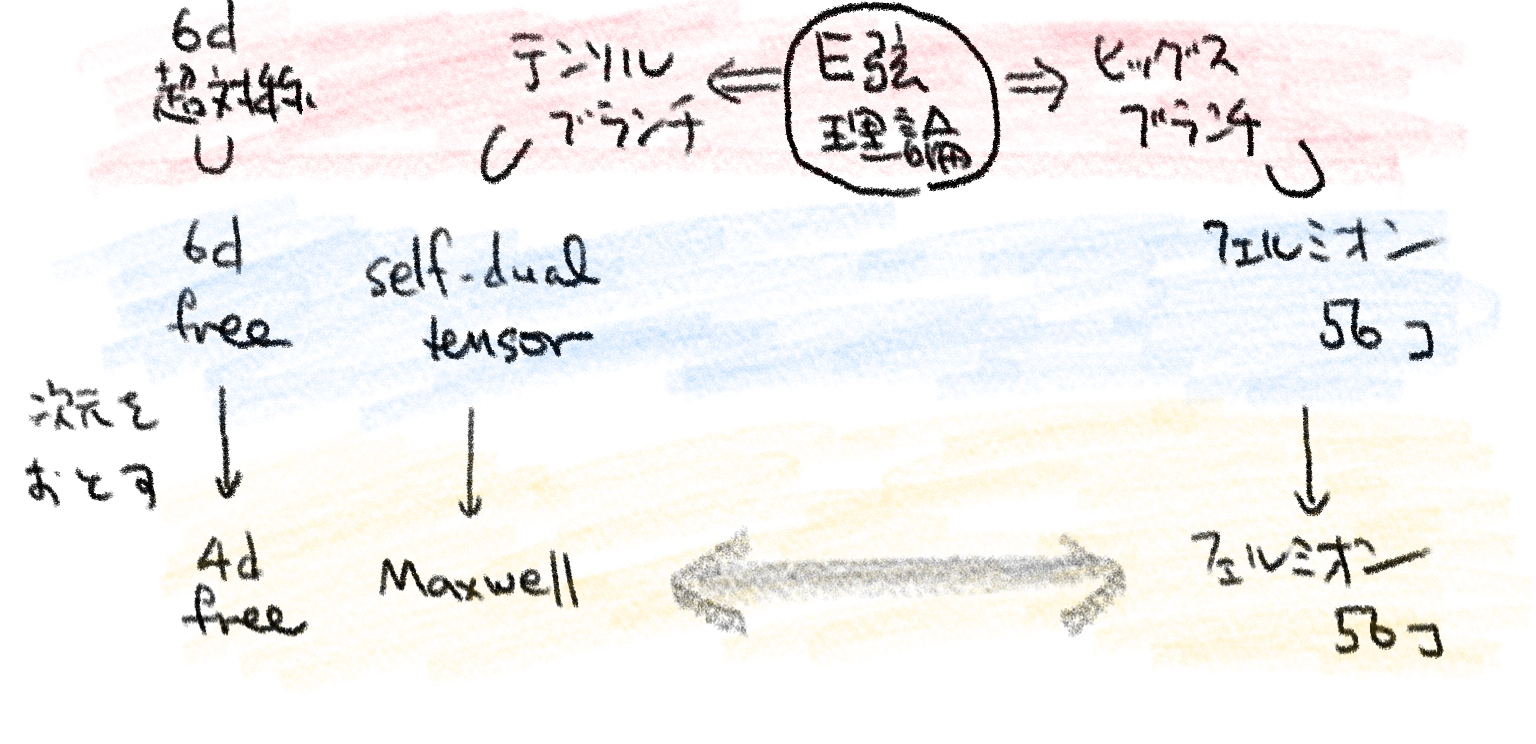
\includegraphics[width=1\textwidth]{pic24}
\]
\end{frame}

\begin{frame}
E-string 理論は非自明な六次元超対称共形場理論で一番小さいもので、僕は五年ぐらいまえから全然別の動機で研究していた。

それが急に四次元の単なる Maxwell 理論の性質を理解するのに\\
「役に立った」ので、びっくりしました。

興味を持った人は、僕らの論文が出ましたら読んでみてください。\\

\end{frame}

\boo{カイラルフェルミオンと\\
 Chern-Simons に関する補足}

\begin{frame}[label=detail]
考える対称性は電磁気の $U(1)$ 対称性。
ゲージ変換は \[
 A_\mu \to  A_\mu+\frac{1}{2\pi i} e^{-2\pi i\chi}\partial_\mu  e^{2\pi i\chi} = A_\mu + \partial_\mu \chi
\] 
だから\[
\oint A_t dt \to \oint A_t dt + \oint \partial_t \chi dt 
\] $\chi\sim \chi+1$ だから \[
\oint A_t dt \sim \oint A_t dt + 1.
\]
\end{frame}


\begin{frame}
$1+1$ 次元境界のフェルミオンを、
空間方向を円周上において考える。
\[
\inc{pic18}
\]
一粒子エネルギーレベルは \[
E \propto n + \oint A_t dt
\]
負エネルギー状態は Dirac の海。
\end{frame}
\begin{frame}
きちんと正則化すると、Dirac の海は電荷 \[
\green{q = \oint A_t dt }
\] を持つ。
分配関数は \[
Z=\tr e^{-\beta H} e^{ i\green{q} \alert{\oint A_t dt}}
\] だが、ゲージ変換\[
\alert{\oint A_t dt} \to \alert{\oint A_t dt }+\alert{\oint \partial_t \chi dt}
\] のもとで \[
Z \to Z e^{i\green{q}\alert{\oint \partial_t \chi dt}} = Z \exp({i\alert{\oint \partial_t \chi dt}\green{\oint A_t dt}})
\] となってしまう。分配関数の位相が定まらない!
\end{frame}


\begin{frame}
バルクの有効作用は Chern-Simons 項 $e^{iS_\text{CS}}$ ただし \[
S_\text{CS}=\int_{M_3} AdA \propto \int_{M_3} \epsilon^{\mu\nu\rho} A_{\mu} \partial_\rho A_\sigma
\]
ゲージ変換 \[
A\mapsto A+d\chi
\] のもとでの変化は\[
\delta \int_{M_3} AdA = \int_{M_3} d\chi dA 
= \int_{\partial M_3} (d\chi) A.
\]
いまの状況では \[
= \oint \alert{\partial_t\chi dt} \oint \green{A_x dx}
\] で、ちょうど境界のフェルミオンの位相の定まらなさを相殺。

\hyperlink{inflow}{\beamerbutton{本文に戻る}}
\end{frame}

\end{document}
